\documentclass[11pt,a4paper]{report}
\usepackage[utf8]{inputenc}
\usepackage[margin=0.8in]{geometry}
\usepackage{graphicx}
\usepackage[normalem]{ulem}
\useunder{\uline}{\ul}{}
\begin{document}
\begin{center}
\section*{Assignment No. 4}
\end{center}
\rule{\textwidth}{1pt}
\textbf{Aim:}Use of above to draw functional dependency graphs and relevant Software modeling methods, techniques including UML diagrams or other necessities using appropriate tools.
\newline
\rule{\textwidth}{1pt}

\textbf{System Flow Diagram:\\}
\textbf{UML Diagrams:\\}
\section*{Class Diagram:}
\paragraph{}Class diagrams are the most common diagrams used in UML. Class Diagram is main building block of any object oriented solution. It shows the classes in system, at- tributes and operations of each class and the relationship between each class. Class diagram static nature.
\section*{Activity Diagram:}
\paragraph{}It is describes the ow of control in a system. So it consists of activities and links. The flow can be sequential, concurrent or branched. Activities are nothing but functions of the system. It is used to visualize how the system will work when executed.
\begin{figure}[h]
	\centering
	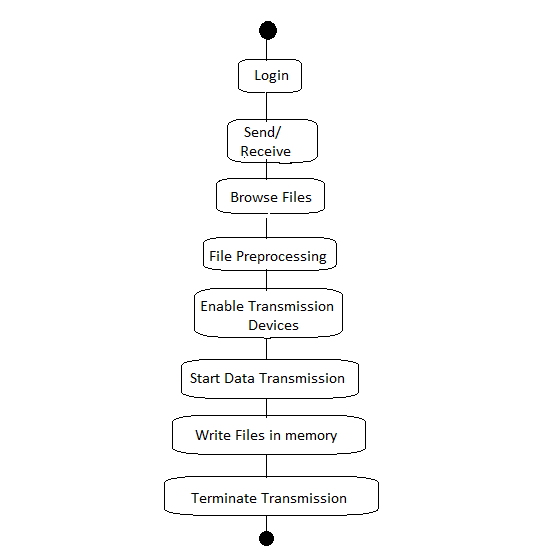
\includegraphics[width=3.5in]{Activity.png}
	\begin{center}\caption{Activity Diagram} \end{center}
	\label{LABEL}
\end{figure}
\section*{Sequence Diagram:}
\paragraph{}The sequence diagram is an interaction diagram. The diagram deals with some sequences, which are the sequence of messages owing from one object to another. Interaction among the component of system is very important from implementation and execution perspective.
\begin{figure}[h]
	\centering
	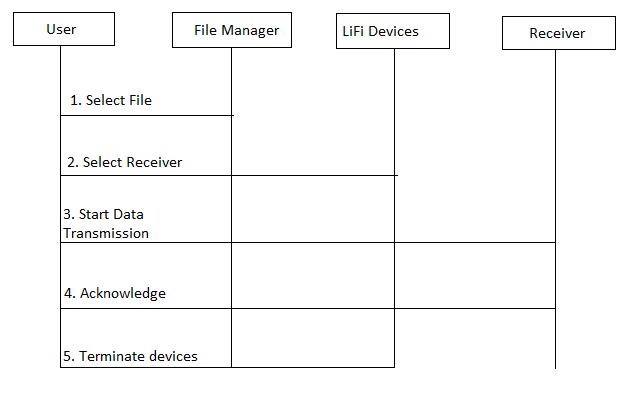
\includegraphics[width=4in]{sequence.png}
	\begin{center}\caption{Sequence Diagram} \end{center}
	\label{LABEL}
\end{figure}
\section*{Use Case Diagram:}
\paragraph{}Use Case diagram are a set of use cases, actors and their relationships. They represent the use case view of a system. A use case represents a particular functionality of a system.
\begin{figure}[h]
	\centering
	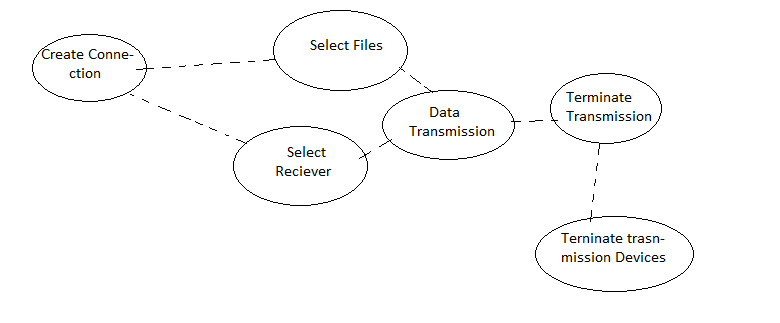
\includegraphics[width=4in]{Use_Case.png}
	\begin{center}\caption{Use Case Diagram} \end{center}
	\label{LABEL}
\end{figure}
\section*{Data Flow Diagram:}
\paragraph{}It is a graphical representation of flow of data through an information system,modeling its process aspects. DFD can also be used for visualization of data processing. A DFD shows what kind of information will be input to and output from the systems.
\begin{figure}[h]
	\centering
	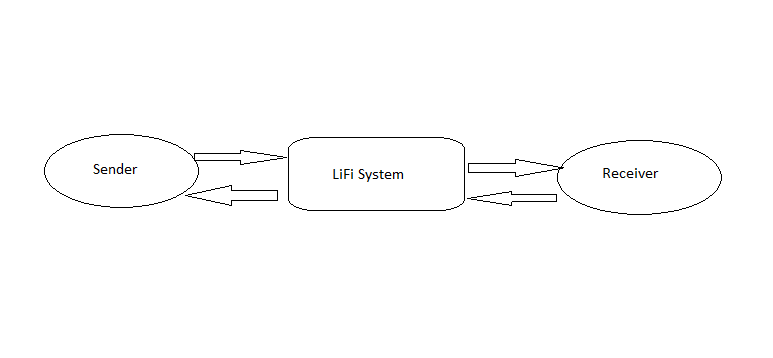
\includegraphics[width=6in]{Data_flow.png}
	\begin{center}\caption{Level  DFD} \end{center}
	\label{LABEL}
\end{figure}
\end{document}